% =============================================================
%  基于非负矩阵分解的神经网络隐藏层表示分析
%  ReLU 与 Tanh 在 MNIST 上的比较研究 —— Beamer 汇报
%  编译：latexmk -xelatex presentation.tex
% =============================================================
\documentclass[aspectratio=169,11pt]{ctexbeamer}

% ---------- 作者信息（请在此处修改） ----------
\newcommand{\InfoAuthor}{作者姓名}
\newcommand{\InfoInstitute}{学校 / 学院}
\newcommand{\InfoDate}{汇报日期}
% ----------------------------------------------

\usepackage{graphicx}
\usepackage{booktabs}
\usepackage{amsmath,amssymb}
\usepackage{tikz}
\usetikzlibrary{arrows.meta,positioning,calc,fit,backgrounds}
\usepackage{pgfplots}
\pgfplotsset{compat=1.18}

% 原始实验图片位于 reports/figures/，以相对路径引用，不复制
\graphicspath{{../../figures/}{../../figures/nmf/}}

% ---------- 配色 ----------
\definecolor{navy}{HTML}{1F3A5F}
\definecolor{navylight}{HTML}{E8EEF5}
\definecolor{accent}{HTML}{C8553D}
\definecolor{graytext}{HTML}{5A5A5A}
\definecolor{relucol}{HTML}{1F77B4}   % 与实验图中 ReLU 颜色一致
\definecolor{tanhcol}{HTML}{FF7F0E}   % 与实验图中 Tanh 颜色一致

% ---------- 主题 ----------
\usetheme{default}
\setbeamertemplate{navigation symbols}{}
\setbeamercolor{frametitle}{fg=white,bg=navy}
\setbeamercolor{title}{fg=navy}
\setbeamercolor{subtitle}{fg=graytext}
\setbeamercolor{structure}{fg=navy}
\setbeamercolor{normal text}{fg=black!85}
\setbeamercolor{block title}{fg=white,bg=navy}
\setbeamercolor{block body}{bg=navylight}
\setbeamercolor{block title alerted}{fg=white,bg=accent}
\setbeamercolor{block body alerted}{bg=accent!8}
\setbeamercolor{alerted text}{fg=accent}
\setbeamertemplate{itemize item}{\textcolor{navy}{\rule[0.25ex]{0.45em}{0.45em}}}
\setbeamertemplate{itemize subitem}{\textcolor{graytext}{--}}
\setbeamertemplate{blocks}[rounded][shadow=false]
\setbeamerfont{frametitle}{size=\large,series=\bfseries}
\setbeamerfont{caption}{size=\scriptsize}

\setbeamertemplate{frametitle}{%
  \nointerlineskip
  \begin{beamercolorbox}[wd=\paperwidth,ht=2.4em,dp=0.9em,leftskip=1.2em]{frametitle}
    \usebeamerfont{frametitle}\insertframetitle
  \end{beamercolorbox}%
}
\setbeamertemplate{footline}{%
  \hbox{%
  \begin{beamercolorbox}[wd=0.85\paperwidth,ht=2.2ex,dp=1ex,leftskip=1.2em]{}%
    \color{graytext}\tiny 非负表示与 NMF：ReLU 与 Tanh 在 MNIST 上的比较
  \end{beamercolorbox}%
  \begin{beamercolorbox}[wd=0.15\paperwidth,ht=2.2ex,dp=1ex,rightskip=1.2em]{}%
    \hfill\color{navy}\tiny\insertframenumber\,/\,\inserttotalframenumber
  \end{beamercolorbox}}%
}

\newcommand{\smallnote}[1]{{\footnotesize\color{graytext}#1}}
\newcommand{\src}[1]{{\tiny\color{graytext}数据来源：\texttt{#1}}}

\title{基于非负矩阵分解的神经网络隐藏层表示分析}
\subtitle{ReLU 与 Tanh 在 MNIST 上的比较研究\\[0.4em]
  \footnotesize Understanding Neural Network Representations through Nonnegative Matrix Factorization:\\
  A Comparative Study of ReLU and Tanh on MNIST}
\author{\InfoAuthor}
\institute{\InfoInstitute}
\date{\InfoDate}

\begin{document}

% =============================================================
% 1. 标题页
% =============================================================
{
\setbeamertemplate{footline}{}
\begin{frame}
  \begin{tikzpicture}[remember picture,overlay]
    \fill[navy] (current page.north west) rectangle ([yshift=-0.55cm]current page.north east);
    \fill[navy] (current page.south west) rectangle ([yshift=0.25cm]current page.south east);
  \end{tikzpicture}
  \vspace{1.2em}
  \titlepage
\end{frame}
}

% =============================================================
% 2. 背景与动机
% =============================================================
\begin{frame}{动机：ReLU 的非负输出与 NMF 的非负约束形式相近}
\begin{columns}[T,onlytextwidth]
\column{0.46\textwidth}
\begin{itemize}\small\setlength{\itemsep}{0.5em}
  \item 深度网络常被视为“黑盒”：分类准确，但中间层表示难以直接解读
  \item 隐藏层激活矩阵是网络对数据的\alert{内部编码}，可以当作普通矩阵分析
  \item ReLU 把负值截断为 0 $\Rightarrow$ 激活矩阵\textbf{非负}
  \item NMF 只允许非负成分相加，常被认为倾向得到“部分—整体”式表示
        \smallnote{(Lee \& Seung, 1999)}
\end{itemize}

\column{0.5\textwidth}
\centering
\begin{tikzpicture}[
  font=\footnotesize,
  box/.style={draw=navy,rounded corners=2pt,minimum height=0.85cm,align=center,line width=0.7pt},
  arr/.style={-{Stealth[length=2mm]},line width=0.8pt,navy}]
  \node[box,minimum width=1.3cm] (x) {输入图像\\$x$};
  \node[box,fill=navy!85,text=white,minimum width=1.6cm,right=0.55cm of x] (h) {隐藏层\\“黑盒”};
  \node[box,minimum width=1.2cm,right=0.55cm of h] (y) {类别\\$\hat y$};
  \draw[arr] (x) -- (h);
  \draw[arr] (h) -- (y);
  \node[box,fill=navylight,below=0.7cm of h,minimum width=3.6cm] (A) {激活矩阵 $A\in\mathbb{R}_{\ge 0}^{N\times 128}$};
  \draw[arr,dashed,accent] (h) -- node[right,text=accent]{提取} (A);
  \node[box,fill=accent!10,draw=accent,below=0.5cm of A,minimum width=3.6cm] (nmf) {NMF：$A\approx WH,\; W,H\ge 0$};
  \draw[arr] (A) -- (nmf);
  \node[below=0.15cm of nmf,text=graytext,align=center] {观察：分布、稀疏性、成分结构、类别关联};
\end{tikzpicture}
\end{columns}
\vspace{0.6em}
\begin{block}{本项目的定位}
\small 以数值实验观察非负激活与 NMF 之间的联系；\textbf{不}主张 ReLU 网络与 NMF 在数学上等价，也\textbf{不}把更高的稀疏性等同于更强的可解释性。
\end{block}
\end{frame}

% =============================================================
% 3. 研究问题
% =============================================================
\begin{frame}{四个研究问题：从激活分布到 NMF 结构}
\centering
\begin{tikzpicture}[
  q/.style={draw=navy,fill=navylight,rounded corners=3pt,minimum width=6.6cm,minimum height=1.55cm,
            text width=6.2cm,align=left,font=\small,line width=0.6pt},
  tag/.style={fill=navy,text=white,font=\bfseries\small,rounded corners=2pt,inner sep=3pt}]
  \node[q] (q1) at (0,0) {ReLU 与 Tanh 的隐藏层激活\\在\textbf{数值分布}上有何差异？};
  \node[q] (q2) at (7.2,0) {ReLU 的非负激活是否表现出\\\textbf{更明显的稀疏性}？};
  \node[q] (q3) at (0,-2.0) {对激活矩阵做 NMF，能否得到\\\textbf{权重分布各不相同}的 components？};
  \node[q] (q4) at (7.2,-2.0) {ReLU 与 Tanh 正值部分的 NMF 在\\\textbf{重构误差与稀疏性}上有何差别？};
  \foreach \n/\t in {q1/RQ1,q2/RQ2,q3/RQ3,q4/RQ4}
    \node[tag,anchor=north west] at ([xshift=-4pt,yshift=6pt]\n.north west) {\t};
\end{tikzpicture}

\vspace{1.0em}
\smallnote{贯穿全程的问题：这些数值现象能在多大程度上帮助我们理解网络的内部表示？}
\end{frame}

% =============================================================
% 4. 数学背景
% =============================================================
\begin{frame}{数学背景：两种激活函数与非负矩阵分解}
\begin{columns}[T,onlytextwidth]
\column{0.42\textwidth}
\centering
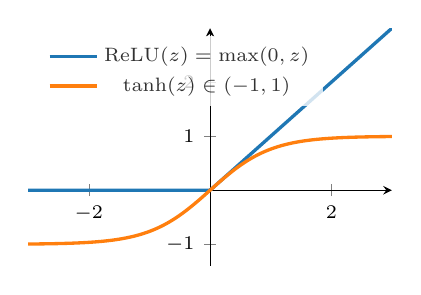
\begin{tikzpicture}
\begin{axis}[
  width=6.2cm,height=4.6cm,
  axis lines=middle,xmin=-3,xmax=3,ymin=-1.4,ymax=3,
  xtick={-2,0,2},ytick={-1,1,2},
  tick label style={font=\scriptsize},
  legend style={font=\scriptsize,at={(0.03,0.97)},anchor=north west,draw=none,fill=white,fill opacity=0.8},
  samples=200,domain=-3:3]
  \addplot[relucol,very thick] {max(0,x)};
  \addplot[tanhcol,very thick] {tanh(x)};
  \legend{{$\mathrm{ReLU}(z)=\max(0,z)$},{$\tanh(z)\in(-1,1)$}}
\end{axis}
\end{tikzpicture}

\vspace{0.2em}
{\footnotesize
\begin{tabular}{lcc}
\toprule
 & ReLU & Tanh \\
\midrule
值域 & $[0,\infty)$ & $(-1,1)$ \\
精确零值 & 有（$z\le 0$） & 仅 $z=0$ \\
饱和 & 仅负半轴 & 两端饱和 \\
\bottomrule
\end{tabular}}

\column{0.54\textwidth}
\begin{block}{非负矩阵分解（NMF）}
给定非负矩阵 $A\in\mathbb{R}_{\ge0}^{N\times d}$ 与秩 $k$：
\[
  \min_{W\ge 0,\;H\ge 0}\ \tfrac12\,\|A-WH\|_F^2,\qquad
  W\in\mathbb{R}^{N\times k},\ H\in\mathbb{R}^{k\times d}
\]
\end{block}
\vspace{0.3em}
\begin{itemize}\setlength{\itemsep}{0.35em}
  \item 每一行（样本）被写成 $k$ 个非负成分的\textbf{加权叠加}：
        $a_i\approx\sum_{j=1}^{k} w_{ij}\,h_j$
  \item 因系数与成分均非负，成分之间\alert{只能相加，不能相互抵消}
  \item 这一“加性”直觉是本项目的出发点，而\textbf{不是}结论
\end{itemize}
\end{columns}
\end{frame}

% =============================================================
% 5. 实验设计
% =============================================================
\begin{frame}{实验设计：仅激活函数不同的成对对照}
\centering
\begin{tikzpicture}[
  font=\footnotesize,
  lay/.style={draw=navy,rounded corners=2pt,minimum height=1.0cm,align=center,line width=0.7pt,fill=white},
  arr/.style={-{Stealth[length=2mm]},line width=0.8pt,navy}]
  \node[inner sep=0] (img) {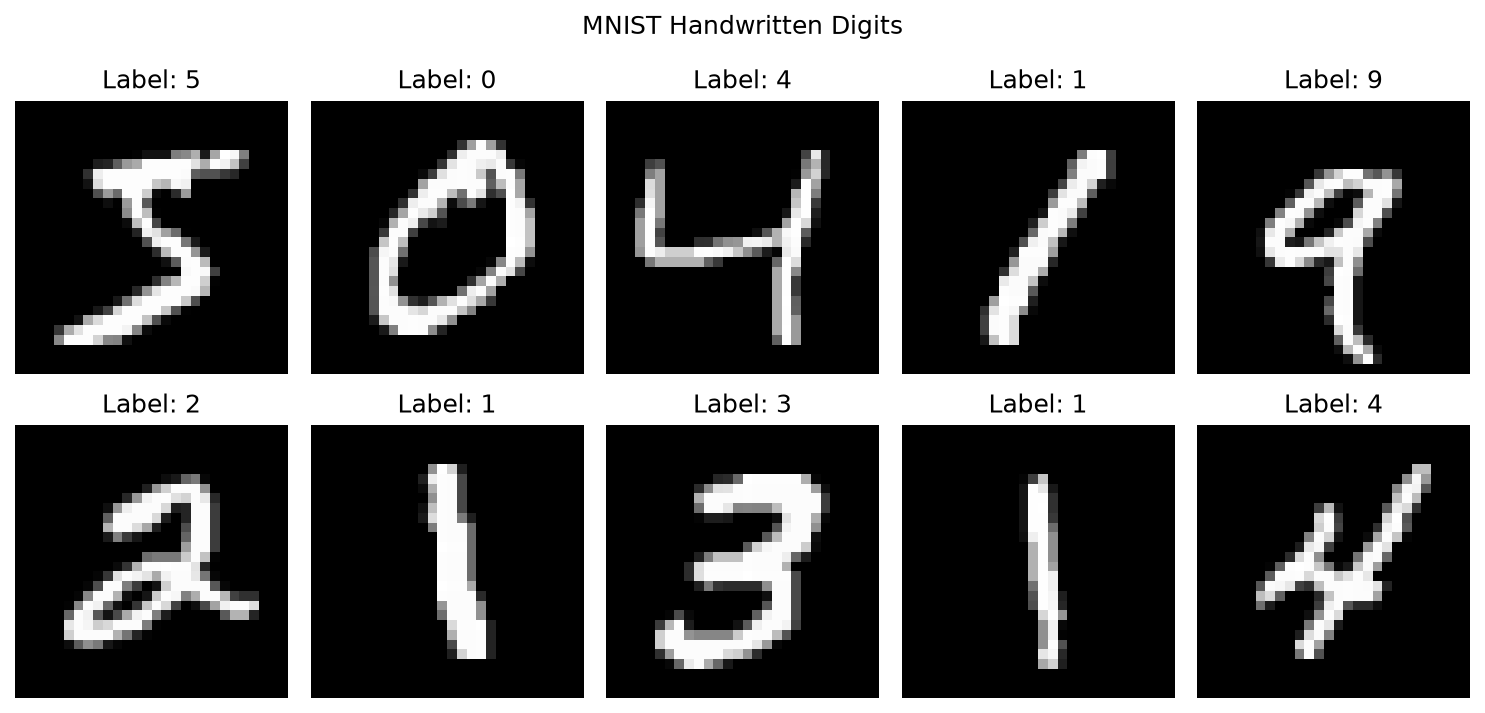
\includegraphics[height=1.75cm]{mnist_samples.png}};
  \node[below=0pt of img,font=\scriptsize,text=graytext] {MNIST 样本，$28\times28$ 灰度};
  \node[lay,right=0.6cm of img] (fl) {Flatten\\784};
  \node[lay,right=0.5cm of fl] (fc1) {Linear\\$784\to128$};
  \node[lay,right=0.5cm of fc1,fill=navylight,minimum width=1.7cm] (act) {\textcolor{relucol}{\textbf{ReLU}}\\或 \textcolor{tanhcol}{\textbf{Tanh}}};
  \node[lay,right=0.5cm of act] (fc2) {Linear\\$128\to10$};
  \node[lay,right=0.5cm of fc2] (out) {logits\\10 类};
  \draw[arr] (img) -- (fl); \draw[arr] (fl) -- (fc1); \draw[arr] (fc1) -- (act);
  \draw[arr] (act) -- (fc2); \draw[arr] (fc2) -- (out);
  \node[draw=accent,dashed,rounded corners=2pt,below=0.55cm of act,fill=accent!8,align=center,font=\scriptsize] (A)
       {隐藏层激活 $A$\\测试集 $10000\times128$};
  \draw[arr,accent,dashed] (act) -- (A);
\end{tikzpicture}

\vspace{0.6em}
\begin{columns}[T,onlytextwidth]
\column{0.5\textwidth}
\begin{block}{训练配置（取自 \texttt{train\_models.py}）}
\footnotesize
\begin{tabular}{@{}ll@{}}
数据 & MNIST：训练 60000 / 测试 10000 \\
预处理 & \texttt{ToTensor()}，像素缩放至 $[0,1]$ \\
优化 & Adam，学习率 $10^{-3}$，batch 128 \\
损失 / 轮数 & 交叉熵 / 5 epochs \\
参数量 & 101{,}770（两模型相同）
\end{tabular}
\end{block}
\column{0.46\textwidth}
\begin{block}{对照设计}
\footnotesize
\begin{itemize}
  \item 两个模型共享\textbf{同一组初始权重}（种子 42）
  \item 训练数据顺序相同（同一随机生成器）
  \item 激活在\textbf{全部测试集}上提取，标签对齐
\end{itemize}
\end{block}
\end{columns}
\end{frame}

% =============================================================
% 6. 分类性能
% =============================================================
\begin{frame}{两种网络分类性能相近：测试准确率相差 0.30 个百分点}
\begin{columns}[c,onlytextwidth]
\column{0.55\textwidth}
\centering
\begin{tikzpicture}
\begin{axis}[
  width=8.2cm,height=5.6cm,
  xlabel={Epoch},ylabel={测试准确率},
  xtick={1,2,3,4,5},ymin=0.925,ymax=0.975,
  yticklabel style={/pgf/number format/fixed,/pgf/number format/precision=3},
  tick label style={font=\scriptsize},label style={font=\small},
  grid=major,grid style={gray!20},
  legend style={font=\small,at={(0.97,0.05)},anchor=south east}]
  \addplot[relucol,very thick,mark=*] coordinates {(1,0.9360)(2,0.9552)(3,0.9645)(4,0.9678)(5,0.9713)};
  \addplot[tanhcol,very thick,mark=square*] coordinates {(1,0.9322)(2,0.9506)(3,0.9614)(4,0.9644)(5,0.9683)};
  \legend{ReLU,Tanh}
\end{axis}
\end{tikzpicture}

\src{reports/metrics/training\_results.json}

\column{0.42\textwidth}
\centering
{\small
\begin{tabular}{lrr}
\toprule
第 5 轮指标 & \textcolor{relucol}{ReLU} & \textcolor{tanhcol}{Tanh} \\
\midrule
测试准确率 & 0.9713 & 0.9683 \\
测试损失 & 0.0955 & 0.1070 \\
训练损失 & 0.0845 & 0.0944 \\
训练时间 (s) & 38.57 & 39.22 \\
\bottomrule
\end{tabular}}

\vspace{1.0em}
\begin{alertblock}{解读注意}
\footnotesize 每种模型\textbf{只训练了一次}，0.30 个百分点的差距不能视为统计显著；训练时间包含每轮测试评估，运行设备未记录。
\end{alertblock}
\end{columns}
\end{frame}

% =============================================================
% 7. 原始激活分布
% =============================================================
\begin{frame}{原始激活：ReLU 集中于零点，Tanh 向 $\pm1$ 两端饱和}
\centering
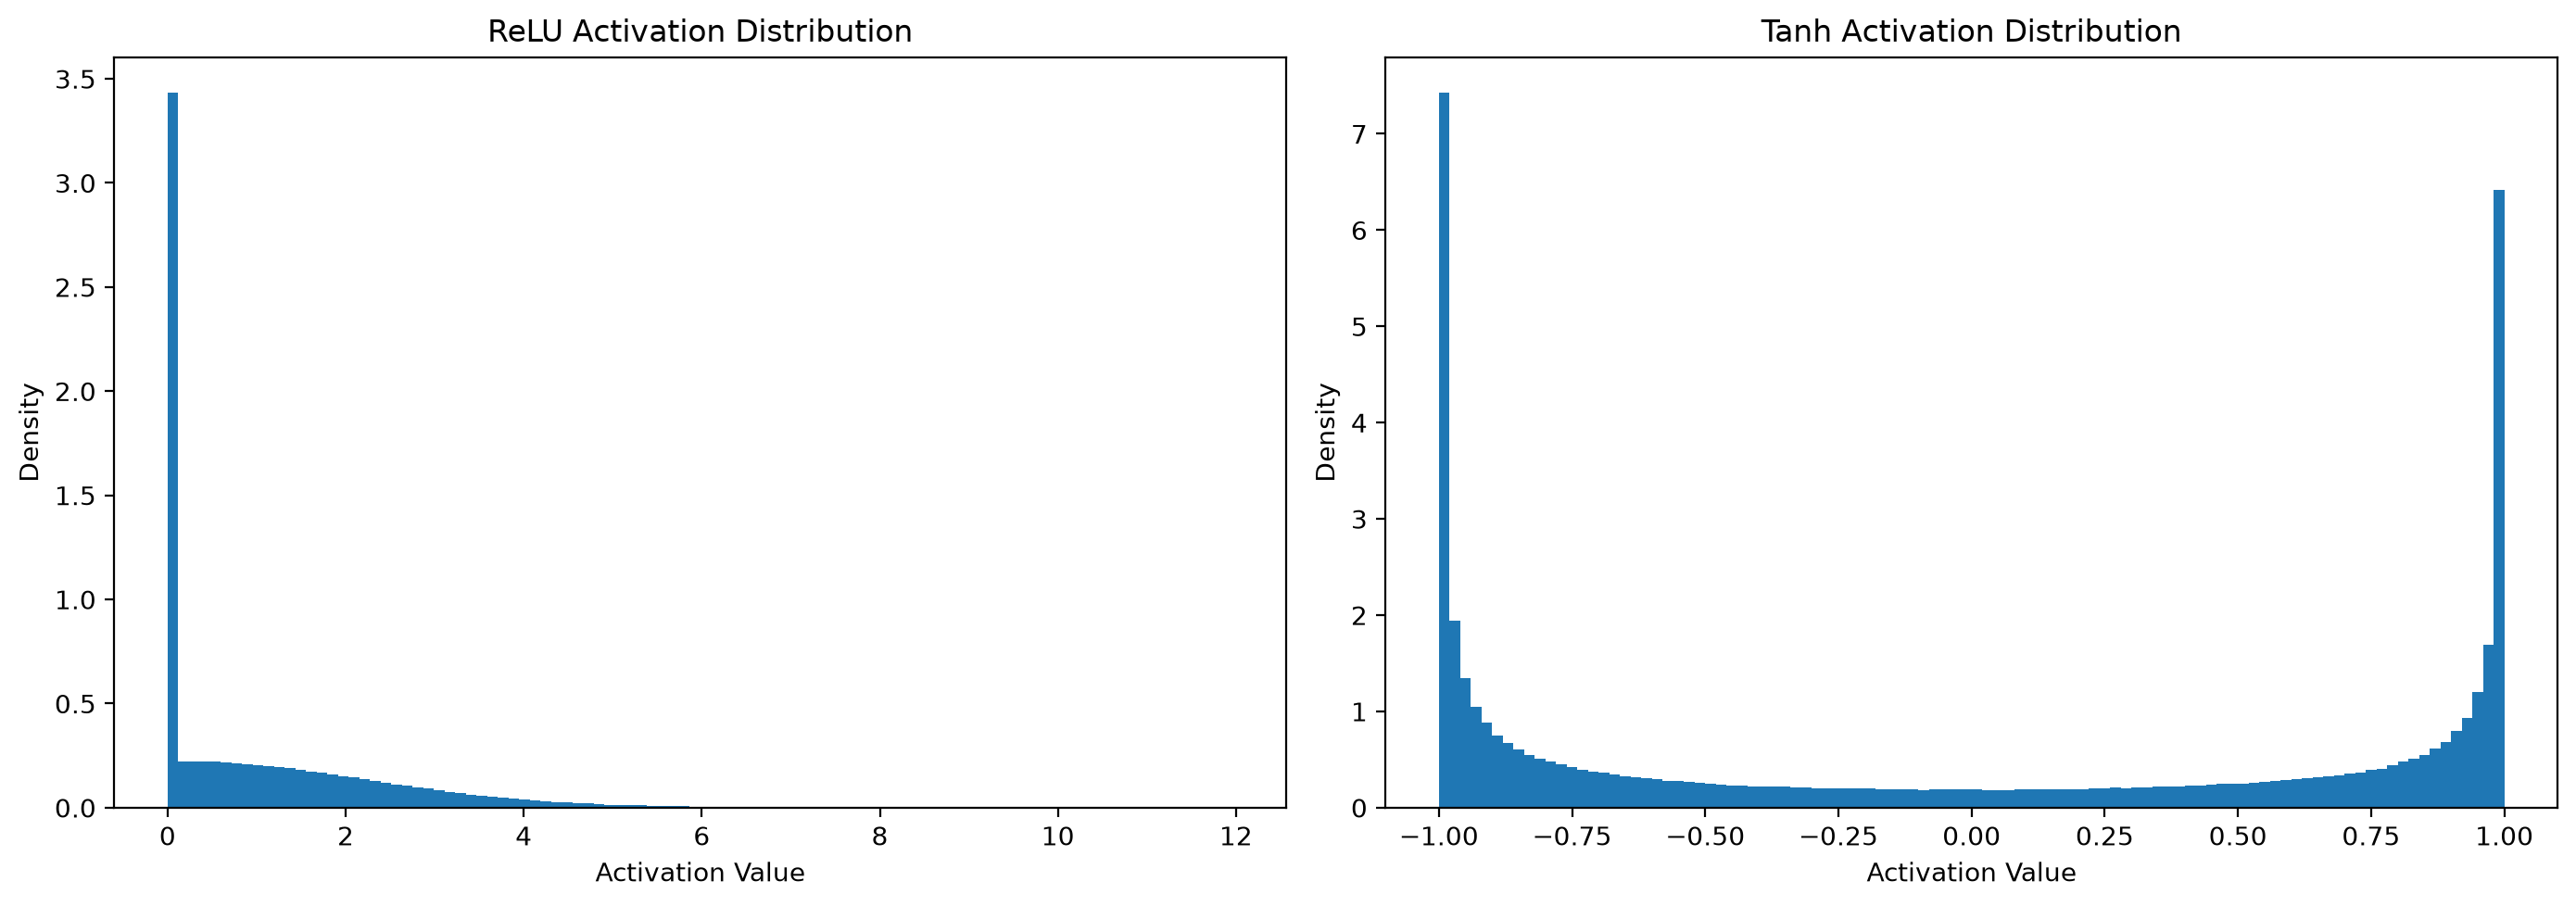
\includegraphics[width=0.92\textwidth]{activation_distributions.png}

\vspace{0.3em}
\begin{columns}[T,onlytextwidth]
\column{0.48\textwidth}
\begin{itemize}\small
  \item \textcolor{relucol}{\textbf{ReLU}}：38.43\% 的激活\textbf{恰好为 0}；正值部分右偏长尾，最大值 11.97
\end{itemize}
\column{0.48\textwidth}
\begin{itemize}\small
  \item \textcolor{tanhcol}{\textbf{Tanh}}：U 形分布，52.16\% 为负；$|a|>0.95$ 的比例平均为 37.7\%
\end{itemize}
\end{columns}
\src{reports/activations/activation\_statistics.json；reports/metrics/neuron\_summary.json}
\end{frame}

% =============================================================
% 8. 原始激活稀疏性
% =============================================================
\begin{frame}{稀疏性：ReLU 有大量精确零值，Tanh 的幅度更“均匀”}
\begin{columns}[T,onlytextwidth]
\column{0.5\textwidth}
\centering
{\small
\begin{tabular}{lrr}
\toprule
指标（$10000\times128$） & \textcolor{relucol}{ReLU} & \textcolor{tanhcol}{Tanh} \\
\midrule
精确零值比例 & 0.3843 & 0 \\
近零比例 $|a|<0.1$ & 0.4063 & 0.0376 \\
负值比例 & 0 & 0.5216 \\
均值 & 1.0615 & $-0.0398$ \\
标准差 & 1.3272 & 0.8029 \\
平均 $|a|$ & 1.0615 & 0.7510 \\
平均 Hoyer（按样本） & \textbf{0.3960} & 0.0707 \\
\bottomrule
\end{tabular}}

\vspace{0.4em}
\begin{tikzpicture}
\begin{axis}[
  ybar,width=7.0cm,height=3.0cm,bar width=10pt,
  symbolic x coords={精确零值,近零 |a|<0.1,Hoyer},xtick=data,
  ymin=0,ymax=0.5,tick label style={font=\scriptsize},
  enlarge x limits=0.25,
  legend style={font=\scriptsize,at={(0.5,1.02)},anchor=south,legend columns=2,draw=none},
  ymax=0.55,nodes near coords,every node near coord/.append style={font=\tiny,/pgf/number format/fixed,/pgf/number format/precision=2}]
  \addplot[fill=relucol,draw=none] coordinates {(精确零值,0.3843)(近零 |a|<0.1,0.4063)(Hoyer,0.3960)};
  \addplot[fill=tanhcol,draw=none] coordinates {(精确零值,0)(近零 |a|<0.1,0.0376)(Hoyer,0.0707)};
  \legend{ReLU,Tanh}
\end{axis}
\end{tikzpicture}

\column{0.47\textwidth}
\begin{block}{Hoyer Sparsity {\footnotesize(Hoyer, 2004)}}
\[
S(x)=\frac{\sqrt{n}-\|x\|_1/\|x\|_2}{\sqrt{n}-1}\in[0,1]
\]
\footnotesize 只有一个非零元时 $S=1$；所有元素幅度相同时 $S=0$。此处 $n=128$，对每个样本计算后取平均（由 \texttt{activations/*.npz} 计算）。
\end{block}
\begin{alertblock}{两类指标不同}
\footnotesize
\begin{itemize}
  \item Tanh 的 Hoyer 基于 $|a|$：衡量\textbf{幅度集中程度}，不代表存在精确零值
  \item Tanh 低 Hoyer 主要源于饱和：大量 $|a|\approx1$ 使幅度趋于均匀
\end{itemize}
\end{alertblock}
\end{columns}
\end{frame}

% =============================================================
% 9. NMF 方法
% =============================================================
\begin{frame}{NMF 方法：ReLU 直接分解，Tanh 仅取正值部分}
\centering
\begin{tikzpicture}[font=\scriptsize]
  % A
  \fill[relucol!20,draw=navy] (0,0) rectangle (1.3,1.7);
  \node at (0.65,0.85) {\large $A$};
  \node[right,align=left] at (-2.6,0.85) {$10000\times128$\\样本 $\times$ 神经元};
  \node at (1.75,0.85) {\large $\approx$};
  % W
  \fill[navy!15,draw=navy] (2.2,0) rectangle (2.7,1.7);
  \node at (2.45,0.85) {\large $W$};
  \node[below,align=center] at (2.45,0) {$10000\times k$，样本系数};
  \node at (3.1,0.85) {\large $\times$};
  % H
  \fill[accent!20,draw=accent] (3.5,1.2) rectangle (4.8,1.7);
  \node at (4.15,1.45) {\large $H$};
  \node[right,align=left] at (4.95,1.45) {$k\times128$\\神经元空间中的成分};
\end{tikzpicture}

\vspace{0.1em}
\begin{columns}[T,onlytextwidth]
\column{0.48\textwidth}
\begin{block}{两组输入矩阵}
\small
\begin{itemize}
  \item \textcolor{relucol}{\textbf{ReLU}}：$A_{\mathrm{ReLU}}$ 本身非负，直接分解
  \item \textcolor{tanhcol}{\textbf{Tanh Positive}}：
        $A^{+}_{\mathrm{Tanh}}=\max(A_{\mathrm{Tanh}},0)$
\end{itemize}
\vspace{0.2em}
\footnotesize\alert{Tanh Positive 丢弃了全部负值（52.16\% 的元素被置 0），并不是完整的带符号 Tanh 表示。}
\end{block}
\column{0.48\textwidth}
\begin{block}{共同设置（scikit-learn \texttt{NMF}）}
\small
\begin{tabular}{@{}ll@{}}
秩 $k$ & 4, 8, 12, 16, 24, 32, 48, 64 \\
初始化 & \texttt{nndsvda} \\
求解器 & \texttt{cd}（坐标下降） \\
最大迭代 & 500 \\
随机种子 & 42 \\
\end{tabular}

\vspace{0.3em}
\footnotesize 相对重构误差：$\displaystyle \varepsilon_k=\frac{\|A-WH\|_F}{\|A\|_F}$
\end{block}
\end{columns}
\end{frame}

% =============================================================
% 10. NMF 重构结果
% =============================================================
\begin{frame}{重构误差随秩下降；$k\ge8$ 时 ReLU 误差始终更低}
\begin{columns}[c,onlytextwidth]
\column{0.58\textwidth}
\centering
\begin{tikzpicture}
\begin{axis}[
  width=8.8cm,height=6.2cm,
  xlabel={NMF 秩 $k$},ylabel={相对重构误差 $\varepsilon_k$},
  xtick={4,8,12,16,24,32,48,64},ymin=0.13,ymax=0.55,
  tick label style={font=\scriptsize},label style={font=\small},
  grid=major,grid style={gray!20},
  legend style={font=\scriptsize,at={(0.97,0.97)},anchor=north east,cells={anchor=west}}]
  \addplot[relucol,very thick,mark=*] coordinates
    {(4,0.5199)(8,0.4223)(12,0.3704)(16,0.3331)(24,0.2830)(32,0.2458)(48,0.1944)(64,0.1552)};
  \addplot[tanhcol,very thick,mark=square*] coordinates
    {(4,0.5166)(8,0.4442)(12,0.4076)(16,0.3833)(24,0.3498)(32,0.3236)(48,0.2817)(64,0.2426)};
  % 达到 500 次迭代上限的配置
  \addplot[only marks,mark=o,mark size=5pt,black,thick] coordinates
    {(32,0.2458)(64,0.1552)(12,0.4076)(24,0.3498)(32,0.3236)(48,0.2817)(64,0.2426)};
  \legend{ReLU,Tanh Positive,达到 500 次迭代上限}
\end{axis}
\end{tikzpicture}

\src{reports/metrics/nmf\_rank\_comparison.json；tanh\_positive\_nmf\_results.json}

\column{0.39\textwidth}
\begin{itemize}\small\setlength{\itemsep}{0.5em}
  \item 两条曲线均随 $k$ 单调下降，符合“秩越大、近似越精细”的预期
  \item $k=4$：Tanh Positive 略低\\
        \footnotesize（0.5166 vs.\ 0.5199）\small
  \item $k\ge8$：ReLU 均更低，差距随 $k$ 扩大\\
        \footnotesize（$k=64$：0.1552 vs.\ 0.2426）\small
  \item 16 组配置中有 \alert{7 组}迭代次数等于上限 500，可能未完全收敛
\end{itemize}
\vspace{0.3em}
\smallnote{误差更低只说明低秩近似更容易，\textbf{不}等于可解释性更强。}
\end{columns}
\end{frame}

% =============================================================
% 11. NMF Components
% =============================================================
\begin{frame}{ReLU NMF 成分（$k=16$）：各成分集中在不同的神经元子集}
\begin{columns}[c,onlytextwidth]
\column{0.64\textwidth}
\centering
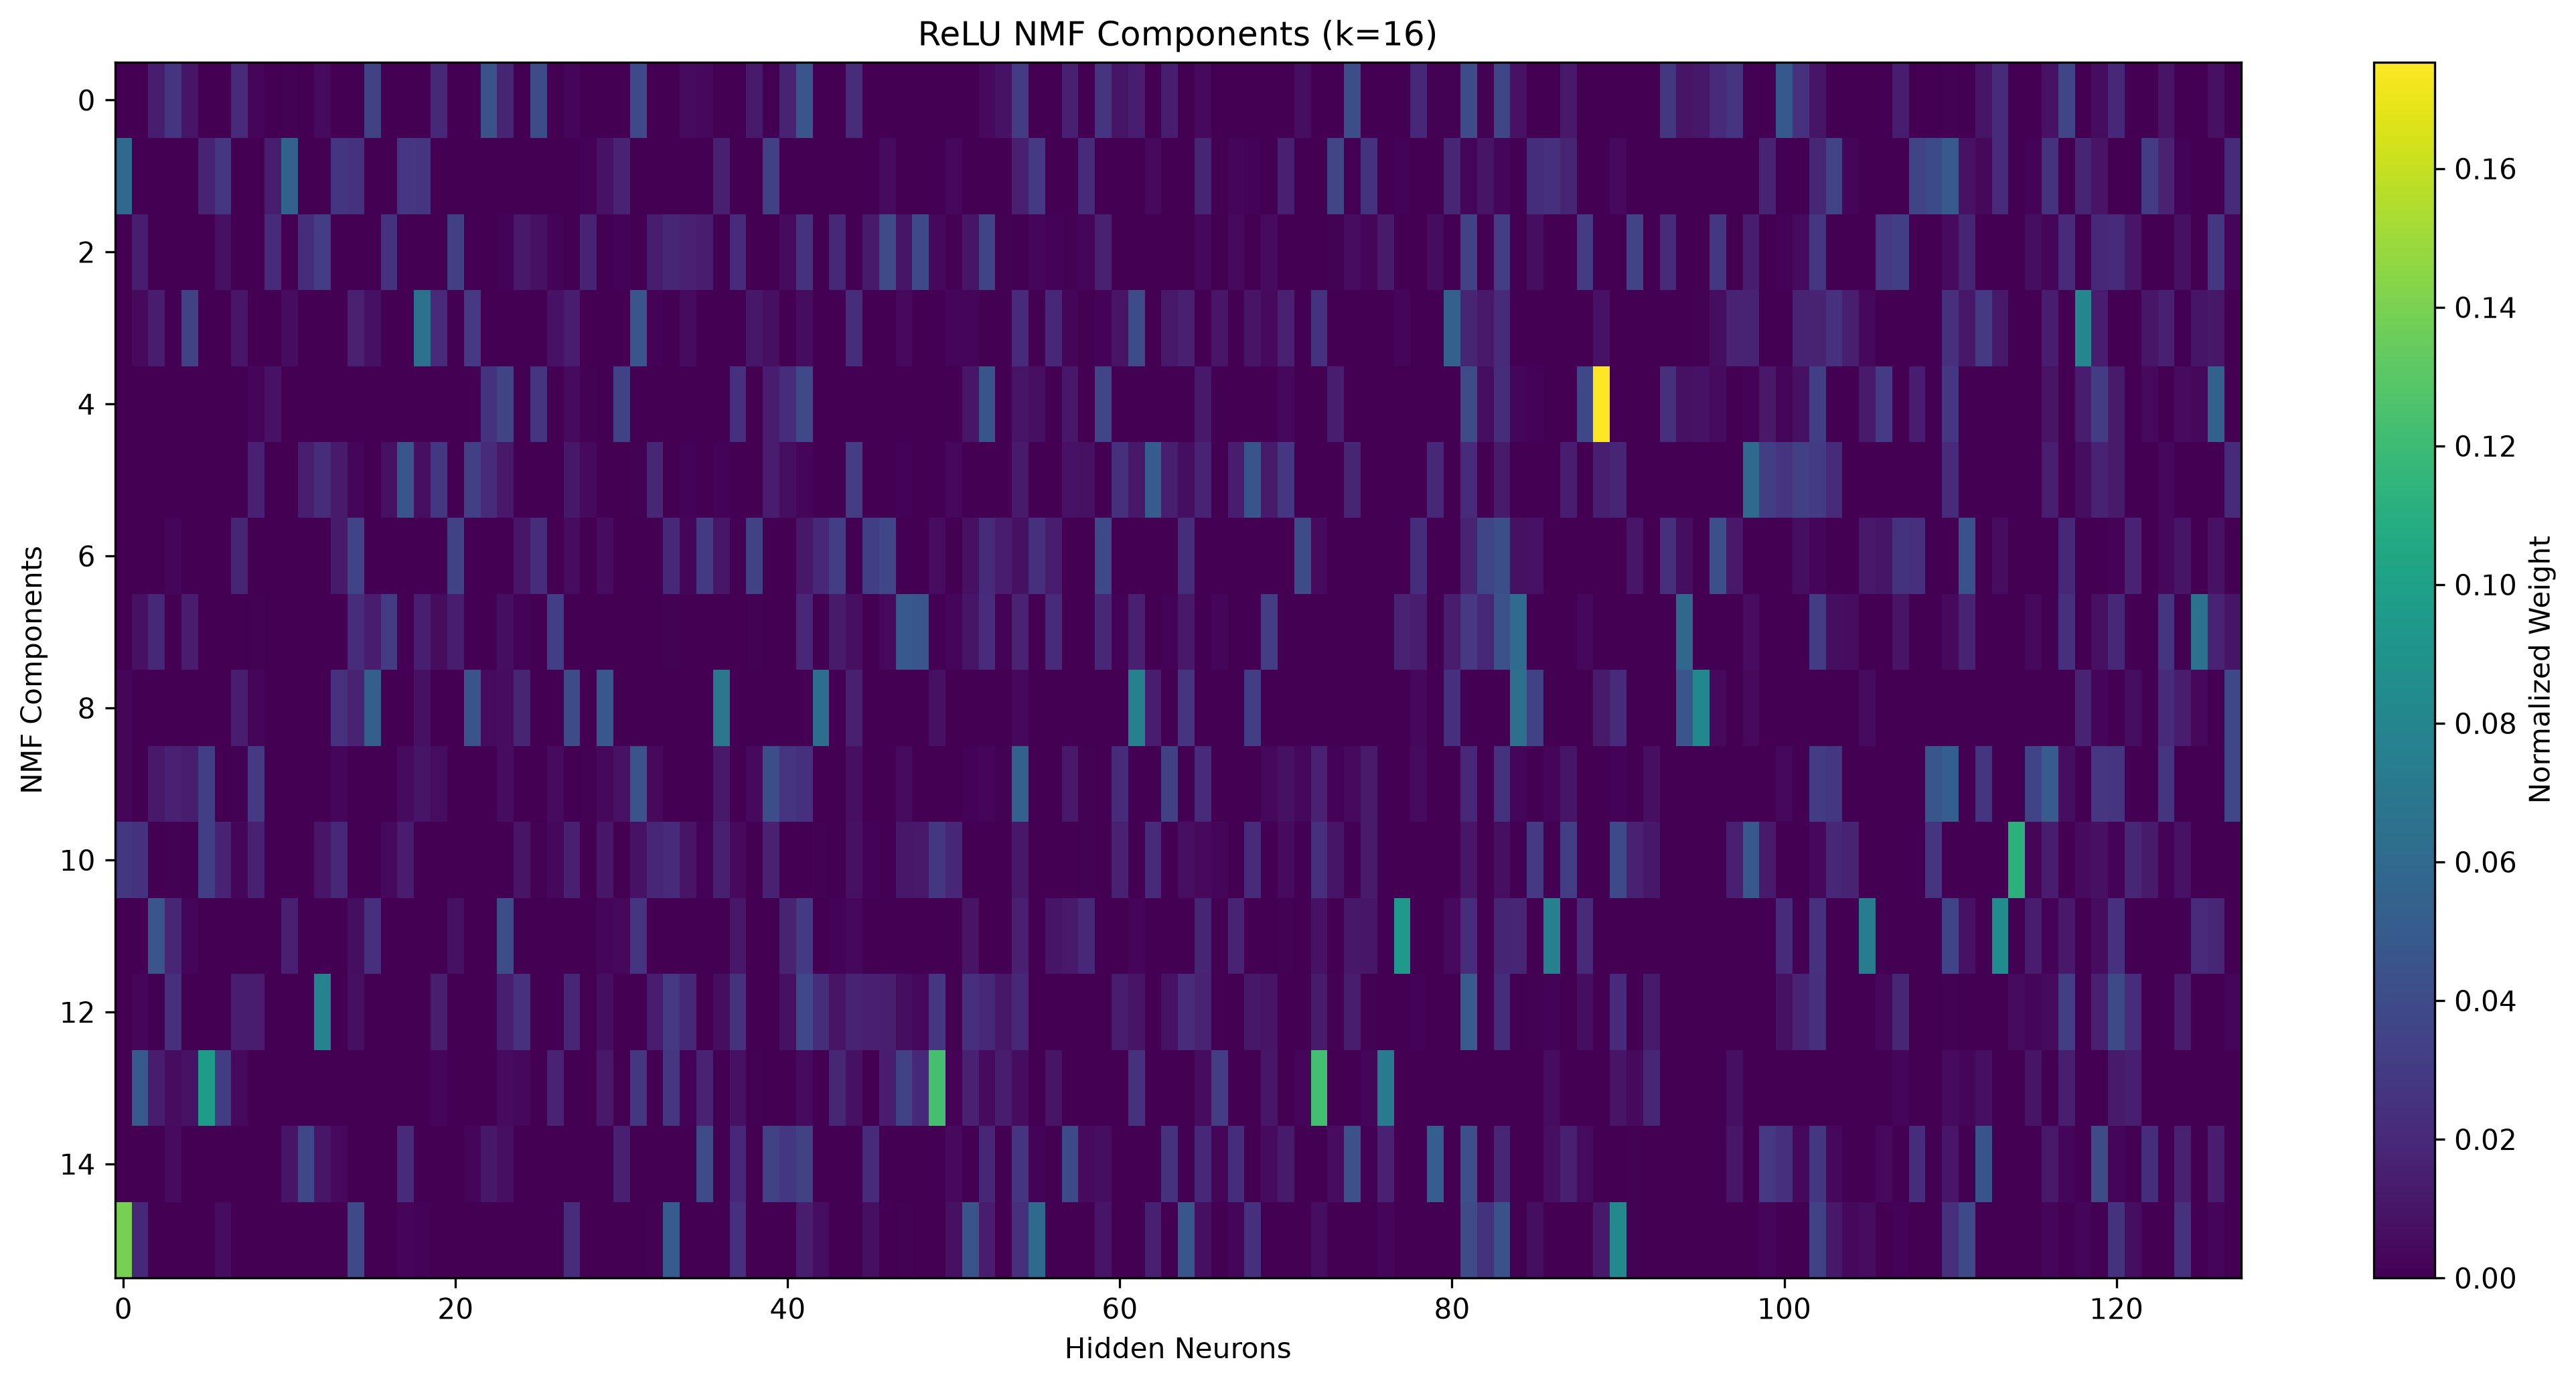
\includegraphics[width=\textwidth]{relu_nmf_components_k16.png}

\smallnote{每行已按行和归一化（行和为 1），以去除成分间的尺度差异。}
\column{0.33\textwidth}
\begin{itemize}\small\setlength{\itemsep}{0.5em}
  \item \textbf{行} = 一个 NMF 成分 $h_j$
  \item \textbf{列} = 128 个隐藏神经元之一
  \item 每个成分只在部分神经元上有明显权重，其余接近 0
  \item 成分 $H$ 的平均 Hoyer：0.5625（范围 0.47–0.69）
\end{itemize}
\vspace{0.4em}
\begin{alertblock}{不是笔画图}
\footnotesize 横轴是神经元编号，\textbf{没有}二维空间排列。此图不能直接读成“横、竖、弯钩”等图像笔画。
\end{alertblock}
\end{columns}
\end{frame}

% =============================================================
% 12. 类别关联
% =============================================================
\begin{frame}{类别关联：每个数字都有响应最强的成分，但多数成分并不专属}
\begin{columns}[c,onlytextwidth]
\column{0.62\textwidth}
\centering
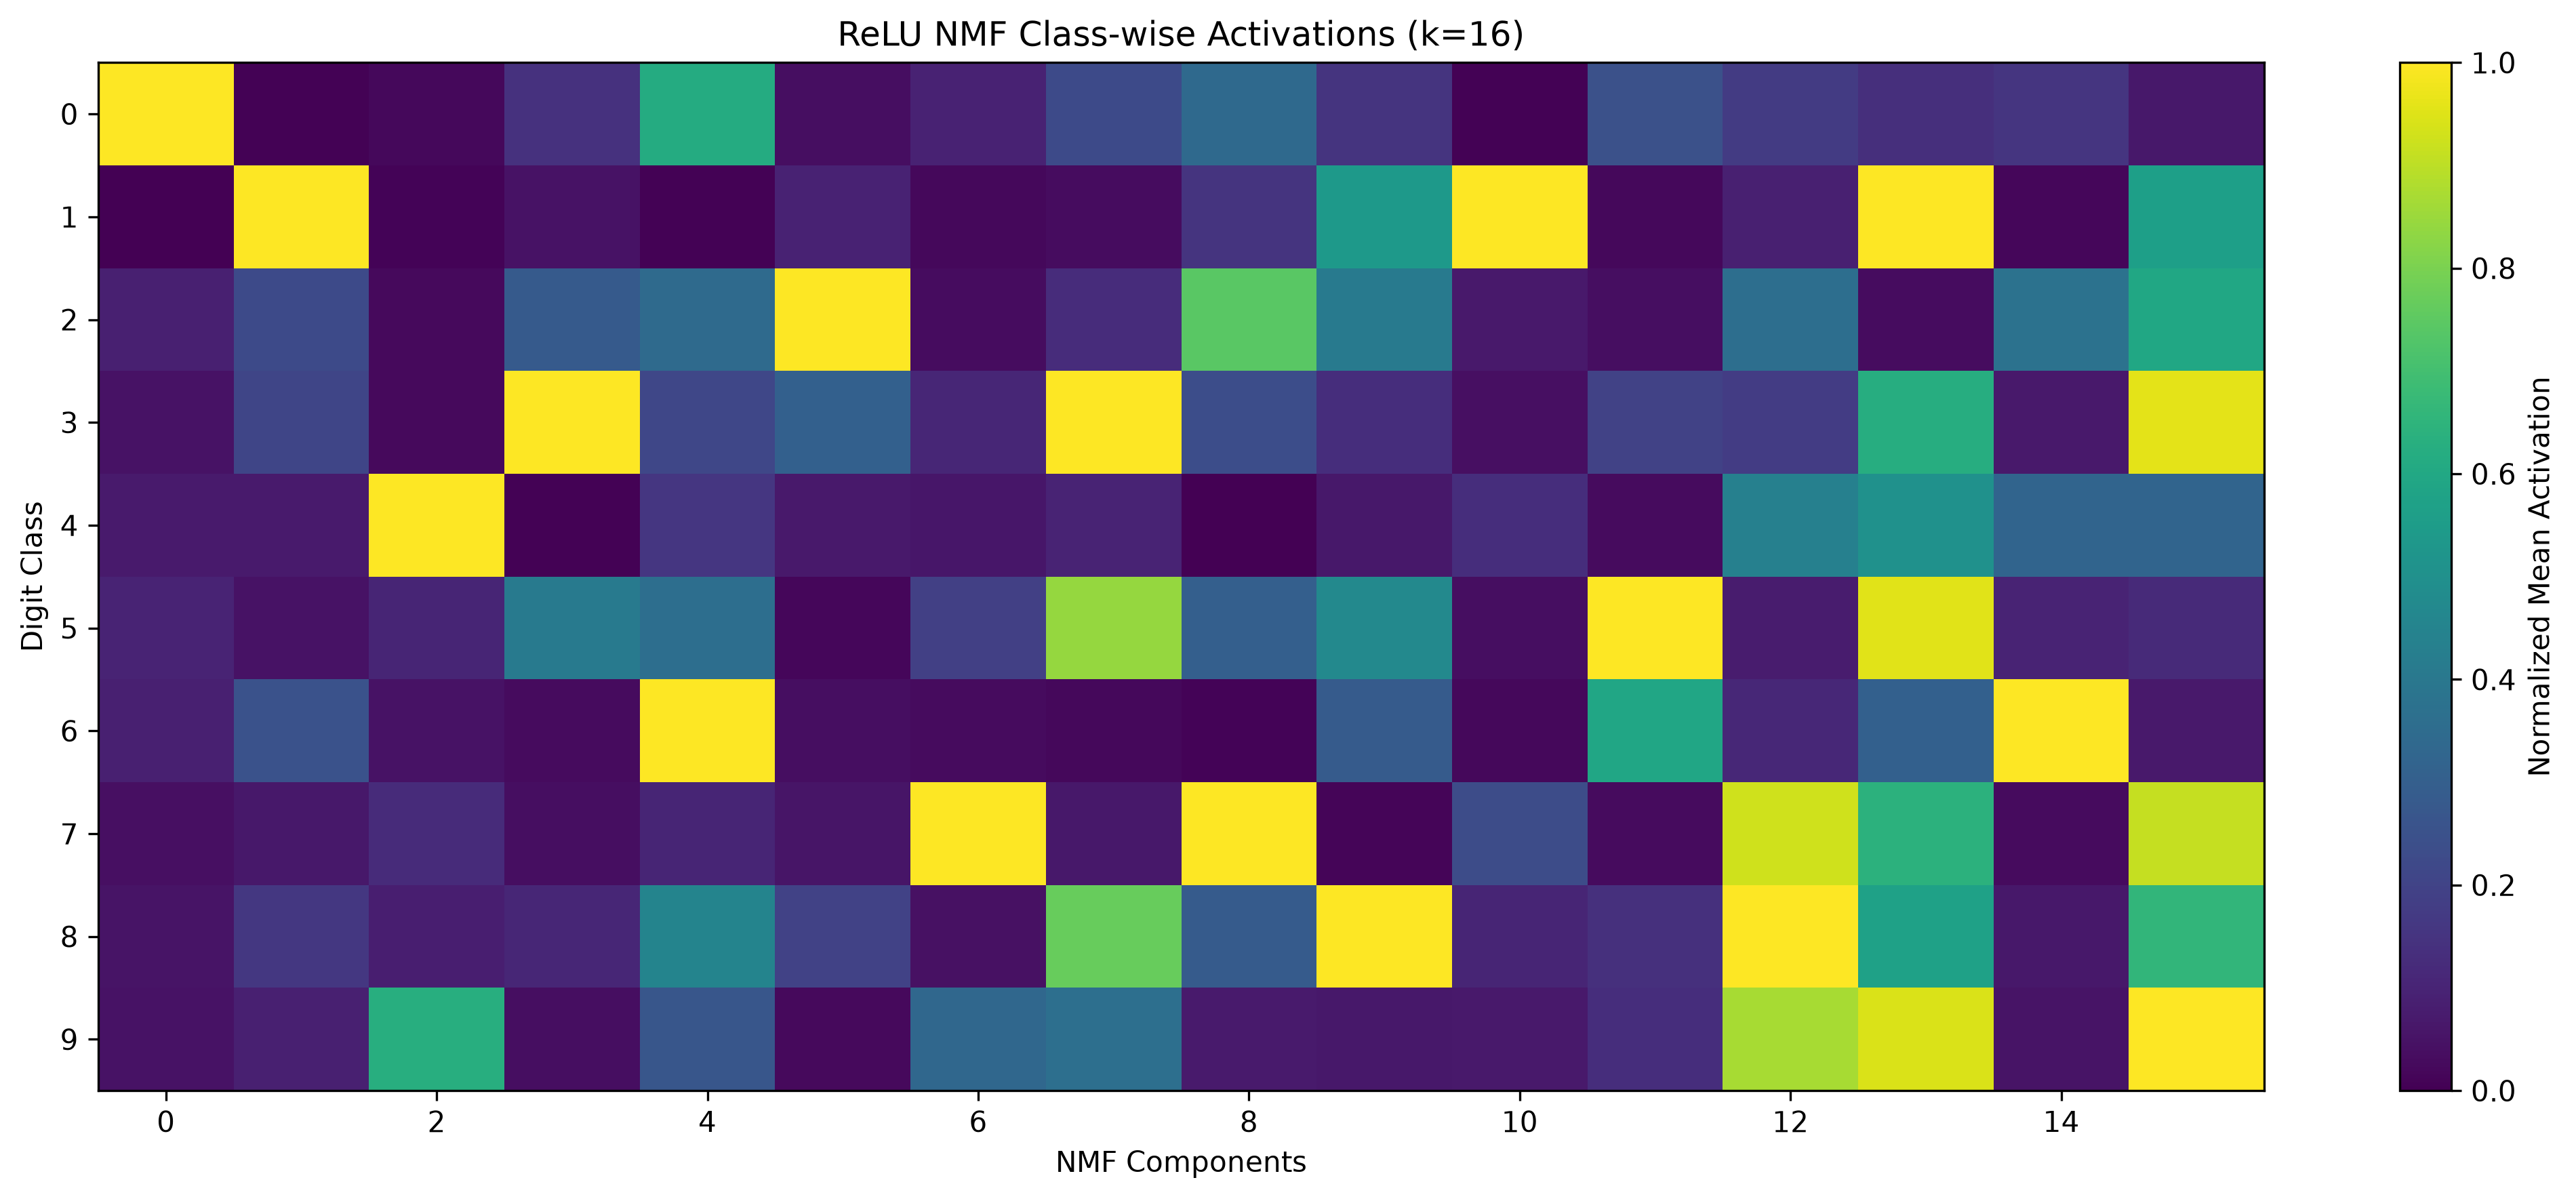
\includegraphics[width=\textwidth]{relu_nmf_class_activation_k16.png}

\smallnote{每格为该类样本在成分上的平均系数 $\bar w_{c,j}$，按列（成分）最大值归一化。}
\column{0.35\textwidth}
\begin{itemize}\small\setlength{\itemsep}{0.45em}
  \item 16 个成分的最强响应类别覆盖了全部 10 个数字
  \item 例：成分 0 主要对应数字 0，成分 2 对应数字 4
  \item 也有成分同时响应多个类别：成分 12 在 7、8、9 上均较强，成分 13 在 1、5、9 上均接近最大值
  \item 最强类与次强类的均值比：中位数 1.77，只有 7/16 个成分超过 2
\end{itemize}
\vspace{0.3em}
\smallnote{这里只是统计上的类别关联，不说明某个成分“专门识别”某个数字。}
\end{columns}
\end{frame}

% =============================================================
% 13. ReLU vs Tanh 定量对比
% =============================================================
\begin{frame}{综合对比：ReLU 的 NMF 误差更低、成分更集中，但优势依赖于秩}
\centering
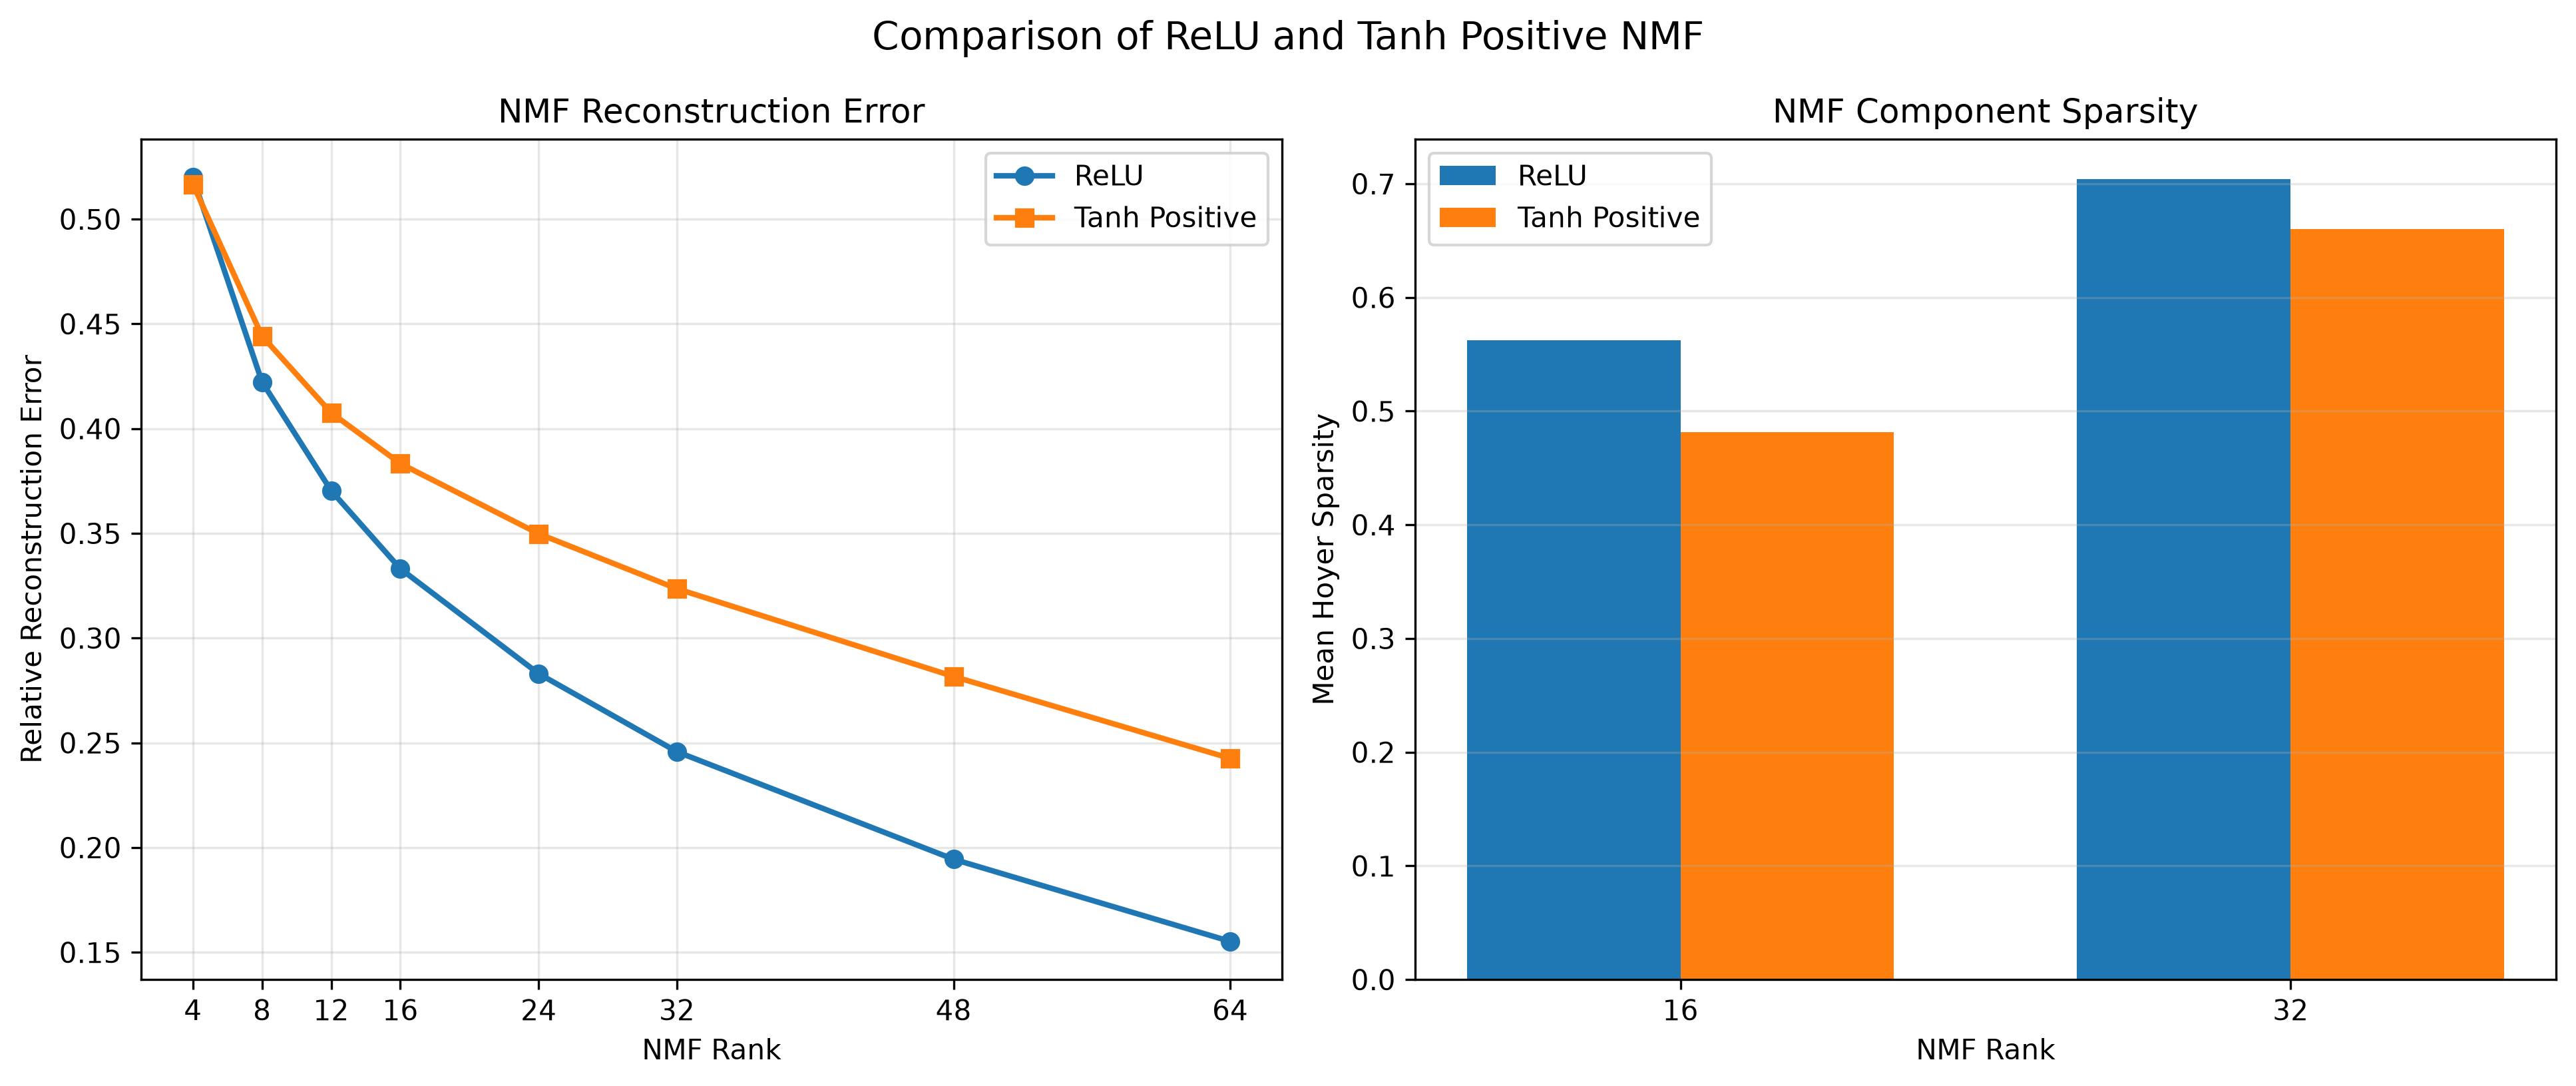
\includegraphics[width=0.72\textwidth]{relu_tanh_nmf_comparison.png}

\vspace{0.2em}
{\footnotesize
\begin{tabular}{lcccccccc}
\toprule
成分 $H$ 平均 Hoyer，$k=$ & 4 & 8 & 12 & 16 & 24 & 32 & 48 & 64 \\
\midrule
\textcolor{relucol}{ReLU} & \textbf{0.367} & \textbf{0.435} & \textbf{0.508} & \textbf{0.563} & \textbf{0.635} & \textbf{0.704} & \textbf{0.783} & 0.841 \\
\textcolor{tanhcol}{Tanh Positive} & 0.354 & 0.418 & 0.456 & 0.481 & 0.582 & 0.660 & 0.769 & \textbf{0.846} \\
\bottomrule
\end{tabular}}

\vspace{0.2em}
\smallnote{原图仅含 $k=16,32$；表中其余秩由已保存的 $H$（\texttt{reports/nmf/*.npz}）计算。$k=64$ 时 Tanh Positive 略高。}
\end{frame}

% =============================================================
% 14. 局限性
% =============================================================
\begin{frame}{局限性：当前证据能支持什么，不能支持什么}
\begin{columns}[T,onlytextwidth]
\column{0.48\textwidth}
\begin{block}{实验设计层面}
\small
\begin{itemize}\setlength{\itemsep}{0.3em}
  \item \textbf{Tanh Positive $\neq$ 完整 Tanh}：负半部分信息全部丢失
  \item Tanh Positive 本身有 52.16\% 的零元素，比 ReLU 的 38.43\% 还多，二者的输入矩阵结构不同
  \item 7/16 个 NMF 配置迭代次数达到上限 500；原始运行日志未保存
  \item 每种激活函数\textbf{只训练一次}，没有方差估计
\end{itemize}
\end{block}
\column{0.48\textwidth}
\begin{block}{解释层面}
\small
\begin{itemize}\setlength{\itemsep}{0.3em}
  \item 稀疏 $\neq$ 可解释：Hoyer 高只说明权重更集中
  \item 隐藏神经元没有空间排列，成分无法直接对应笔画
  \item 按类别关联看，Tanh Positive 成分的最强/次强比更高（$k=16$ 中位数 3.08 vs.\ 1.77），说明 ReLU 并非在所有指标上占优
  \item 结论仅适用于单隐藏层 MLP、MNIST、当前超参数
\end{itemize}
\end{block}
\end{columns}
\end{frame}

% =============================================================
% 15. 总结与展望
% =============================================================
\begin{frame}{总结：非负激活与 NMF 的联系在本实验中可观察，但不构成证明}
\begin{columns}[T,onlytextwidth]
\column{0.58\textwidth}
\begin{block}{观察到的实验事实}
\small
\begin{enumerate}\setlength{\itemsep}{0.25em}
  \item 两种网络测试准确率均约 97\%，差距 0.30 个百分点（单次运行）
  \item ReLU 激活有 38.43\% 精确零值；Tanh 呈两端饱和的 U 形分布
  \item NMF 重构误差随秩单调下降；$k\ge8$ 时 ReLU 误差更低
  \item $k\le48$ 时 ReLU 成分 $H$ 的 Hoyer 更高；$k=64$ 时二者接近
  \item 成分与数字类别存在统计关联，但多数成分不专属于单一类别
\end{enumerate}
\end{block}
\column{0.38\textwidth}
\begin{block}{后续方向}
\small
\begin{itemize}\setlength{\itemsep}{0.3em}
  \item 多随机种子重复训练，给出误差范围
  \item 提高迭代上限，并记录收敛状态
  \item 对 Tanh 采用“正负拆分” $[A^+, A^-]$ 的 NMF，保留完整信息
  \item 将成分映射回输入空间（如加权平均图像），检验其视觉含义
\end{itemize}
\end{block}
\end{columns}
\vspace{0.6em}
\centering
{\color{navy}\bfseries 谢谢！欢迎提问}
\end{frame}

\end{document}
